\chapter{System Design}\label{chapter:general_design_decisions}

\section{Core Design Decisions}
The Framework is designed to be distributed in nature with the concepts of Actors. It should follow the standard actor programming concept and have the inherently distributed nature. The framework itself should be built using the concept of message passing to alleviate any possibility of concurrency issues, thus thread-safe.
\begin{itemize}
  \item The framework does not guarantee the delivery of a message.
  \item All the messages send by the framework is based on ‘fire and forget’concept.
  \item A message is delivered at most once.
  \item A message is always routed through Message Queuing System, even though the target isolate can belong to same isolate system in the same logical or physical node.
  \item A message is only fetched after an isolate sends a PULL request. Nonetheless, the delivery of message to an isolate is based on the implementation of the load balancer \textendash{} i.e. router.
\end{itemize}

\section{Architectural Overview}
\begin{figure}[H]
  \centering
  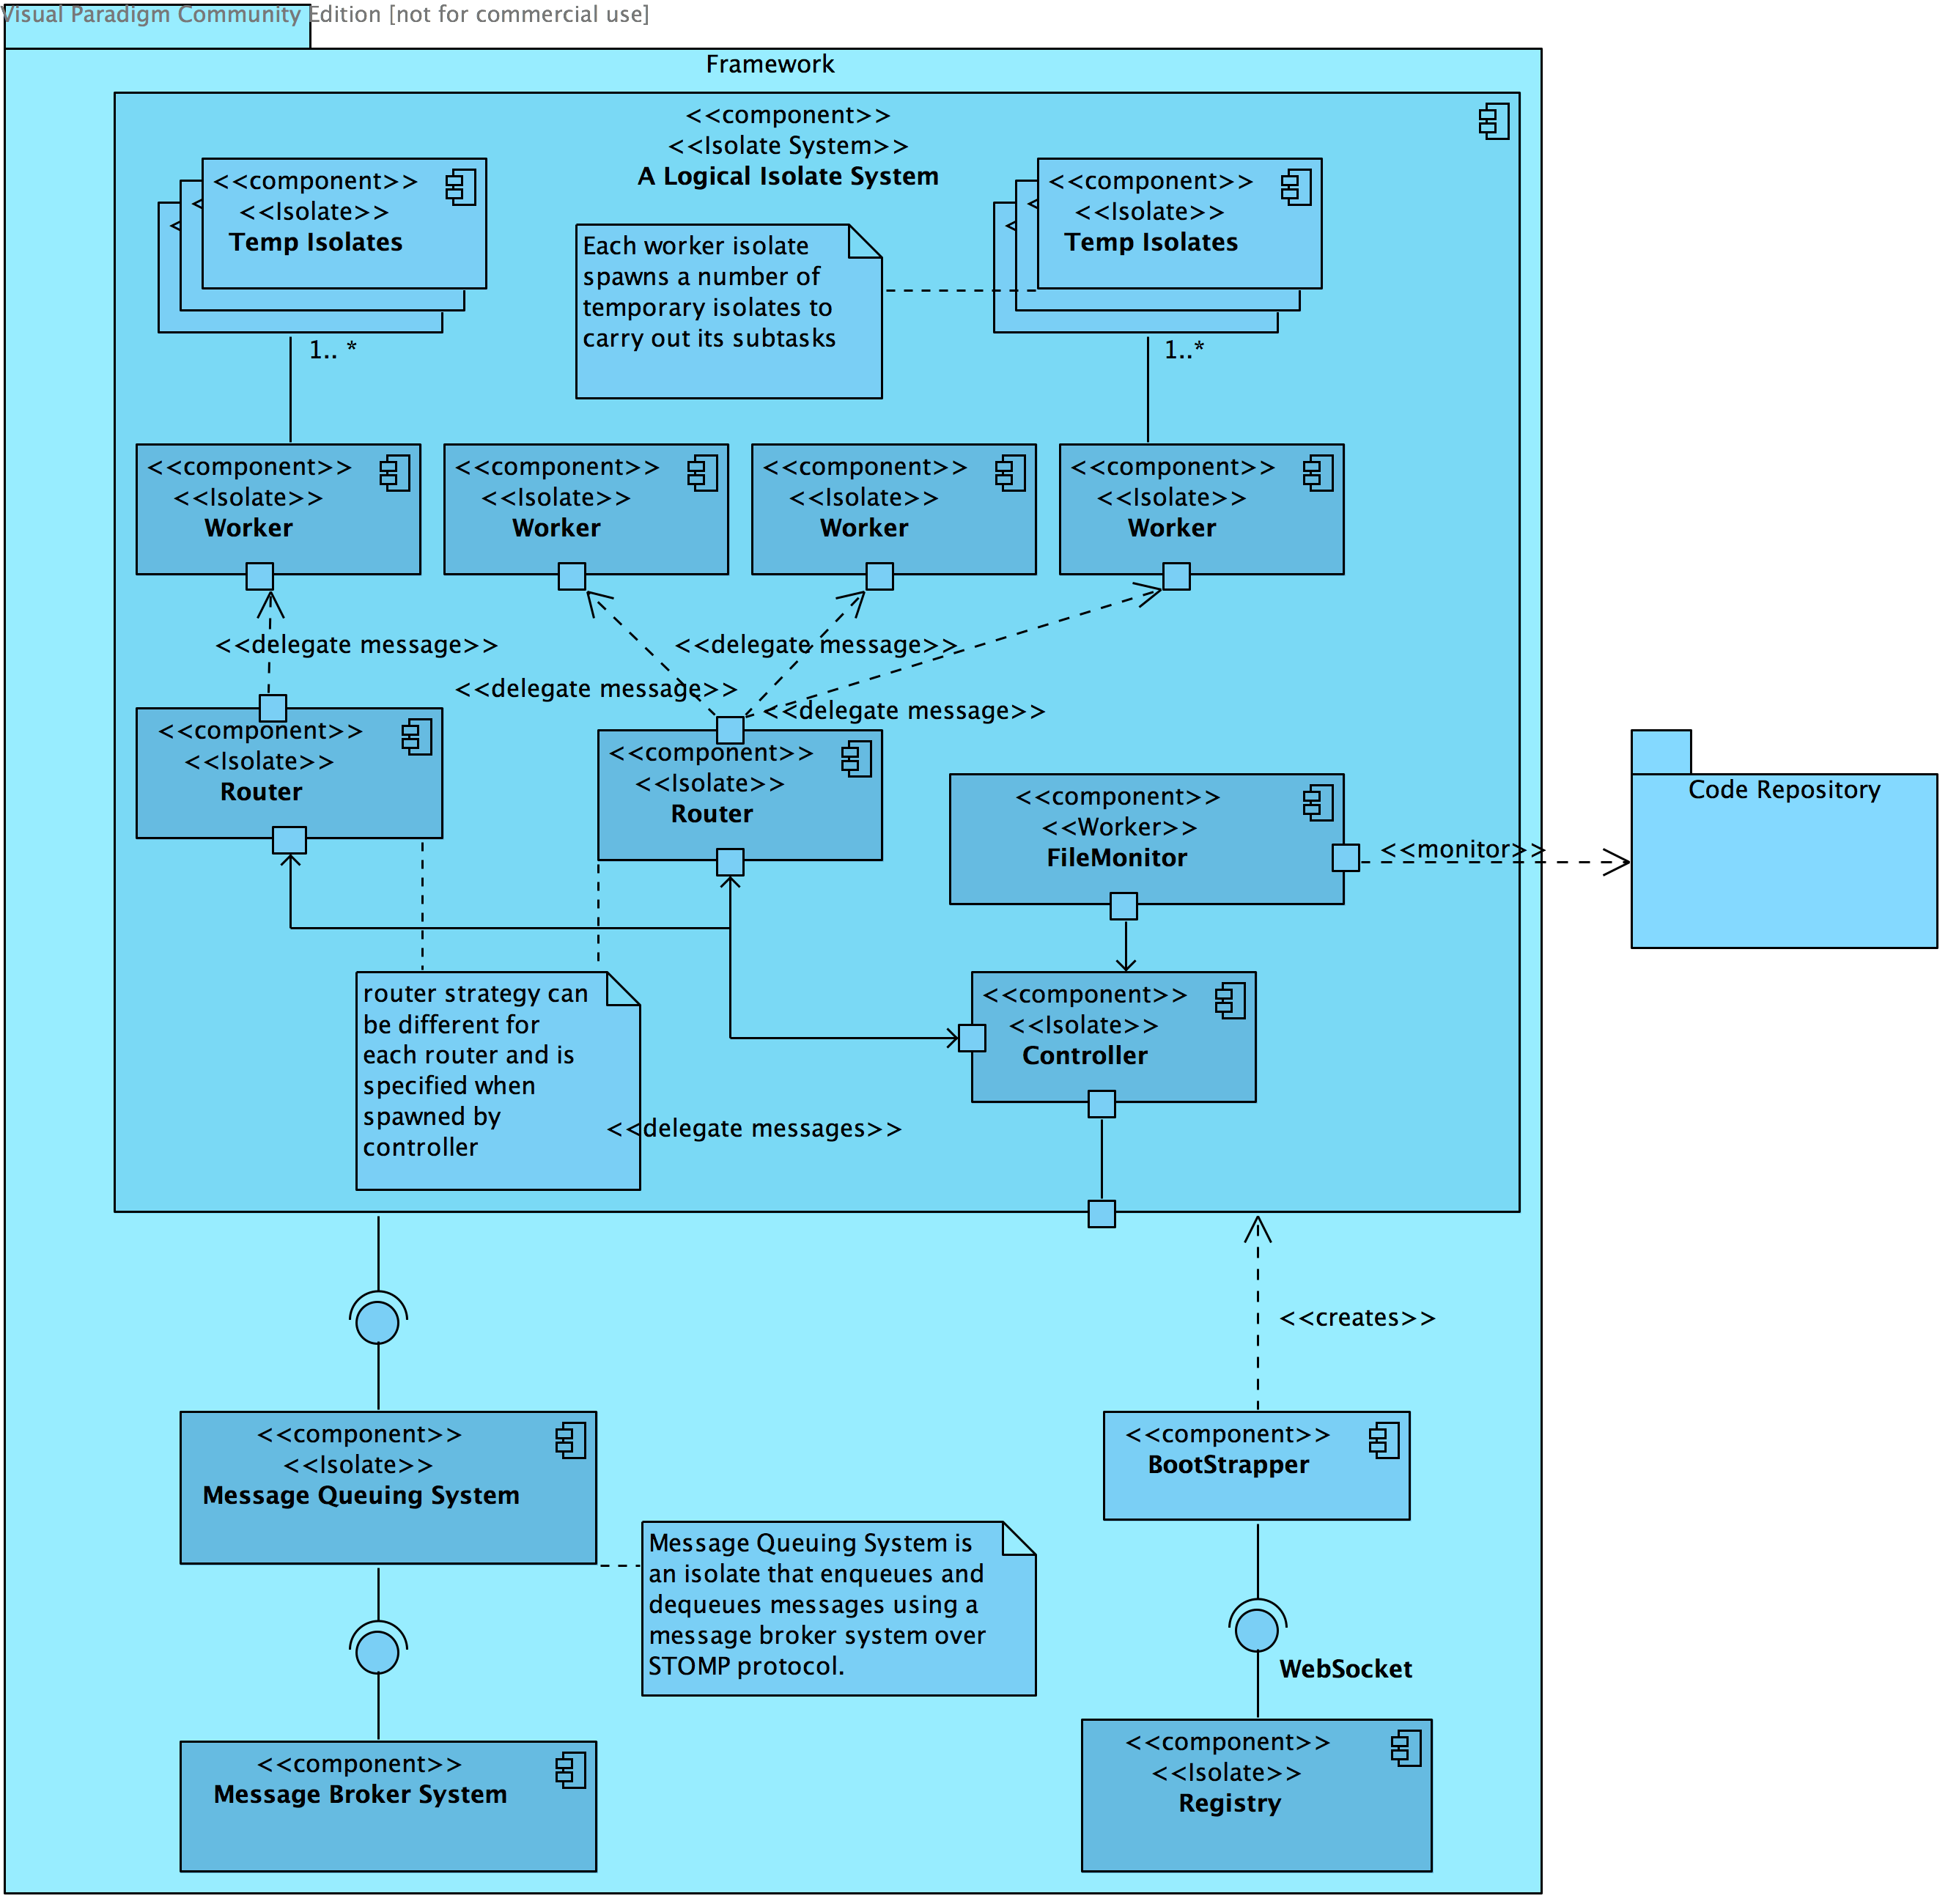
\includegraphics[width=1\textwidth]{figures/componentDiagram}
  \caption[architecture]{Architecture of the framework}
\end{figure}
\section{The Framework}
The framework comprises of an Isolate System, a Registry, a Message Queuing System and a Message Broker System.
  \subsection{IsolateSystem}
  An Isolate System is analogous to an actor system. Just as actor system is comprised of a group of actors working together, a group of related isolates form an isolate system. A ‘Bootstrapper’ in physical node can bootstrap several Isolate Systems. Nevertheless, a logical Isolate System is not limited to a single physical node. The isolates spawned by an Isolate System can be distributed across several remote systems.
  When an Isolate System is bootstrapped, it spawn controller

  \subsubsection{Controller}
  A controller creates routers locally and instructs them to create a certain number of local as well as remote workers with a specific routing policy. Whenever a message arrives in the controller, it delegates the message to the proper router, which then delegates the message to an isolate using the specified routing policy. A Controller handles multiple routers.

  \subsubsection{Router}
  A router is spawned by the controller. It spawns and is responsible for a group of identical workers. Since an isolate is single threaded, multiple instances of an isolate can be created by a router for concurrency. When a message arrives to a router from a controller, the router, based on its defined routing policy, delegates the message to one of the worker isolates.
  For proper load balancing among a group of isolates, a router uses a routing policy. The routing policies that are available in the framework are:

  \begin{description}
    \item{Round Robin Router} Messages are passed in round-robin fashion to child isolates.

    \item{Random Router} Randomly picks an isolate and the message is passed to that isolate.

    \item{Broadcast Router} Replicated and sends message to all child isolates.
  \end{description}

  \subsubsection{Worker}
  Worker isolates carry out the business logic tasks. However, if a certain task is too complex, the isolate can divide the tasks into subtasks and spawn temporary isolates to carry out those subtasks. The temporary isolates, can again spawn other child temporary-isolates to further divide the subtasks into sub-subtask. The temporary isolates terminate once the subtask has been carried out.

  \subsubsection{Proxy}
  A ‘Proxy’ is a special type of Worker. When an isolate is supposed to spawned in a remote node, a proxy isolate is spawned in local node, where the isolate system resides. As the name suggests, the ‘Proxy’ acts as a worker for the router which spawned it but forwards the messages it receives to the remotely spawned isolate via IsolateDeployer. The communication with Isolate Deployer takes place via WebSocket connection where the proxy worker connects as a WebSocket client. Each ‘Proxy’ worker maintains a separate WebSocket connection with an ‘IsolateDeployer’.

  \subsubsection{FileMonitor}
  FileMonitor is also a Worker Isolate. If the ‘Hot Deployement’ flag for an isolate is set while spawning, a ‘FileMonitor’ for that isolate is spawned. The spawned ‘FileMonitor’ monitors the md5 checksum source code of the file from where the Worker Isolate was spawned. If the file is changed, it simply sends the restart command to the controller, which eventually forwards it to the router to restart all of its child isolates.


\subsection{The Registry}
The Isolate Registry is a central registry system where meta-data of isolates and isolate systems are stored. It bootstraps all isolates systems and stores the current deployed location of every isolate system. It’s functions are:
  \subsubsection{RESTful API of Registry}
  The registry provides a REST API to perform the operations on the connected nodes. One can query the ‘Registry’ using the ‘GET’ method of REST to fetch the list of the nodes that are connected to the Registry.
  \begin{itemize}
  \item GET list of connected nodes
  \item GET details of the running isolate systems on the node
  \item POST command to shutdown an isolate system
  \item POST command to kill a particular isolate pool
  \end{itemize}

The functions of Registry are:
\begin{itemize}
  \item Bootstrap an isolate system, during runtime, in local or remote virtual machine
  \item Provide a way to deploy, update or remove an ‘isolate system’
  \item Return information about the isolate systems running isolates by querying the individual isolate systems of a node
\end{itemize}
The registry does not need to persist any data as all the information about isolate systems are queried and generated “on the fly”.

  \subsubsection{Management Interface}
  The deployment of isolates can be managed through the web interface provided by Isolate Registry

\subsection{Message Queuing System (MQS)}
Since, the basis of this system is message passing, the Message Queuing System is an important part of this framework. The Message Queuing System is an isolate that fetches messages from message broker system and dispatches to respective the isolate system, of connected node, where the isolate belongs. Whenever a new isolate system starts up, the isolate system opens up a new WebSocket connection with the message queuing system.
It consists of two major components: Enqueuer \textendash{} which enqueues messages and Dequeuer \textendash{} which dequeues messages
  \subsubsection{Enqueuer}
  Enqueuer is a separate isolate. A Message Queuing System has only one enqueuer, which basically receives message from the MQS and sends message to message broker system \textendash{} RabbitMQ~\ref{sec:rabbitmq} via STOMP~\ref{sec:stomp} protocol.

  \subsubsection{Dequeuer}
  As opposed to Enqueuer, a Message Queuing System maintains several Dequeuers.

\subsection{Activator}
  An activator, basically, brings a node to “life”. It starts up two isolates: Systembootstrapper and IsolateDeployer. Every node that is supposed to be running an Isolate System or become a part of Isolate System by running isolates must be running an Activator. Nevertheless, starting up of SystemBootstrapper and IsolateDeployer separately is also possible.
  \subsubsection{SystemBootstrapper}
When a SystemBootstrapper is started, it registers itself to the ‘Registry’.
  \subsubsection{IsolateDeployer}
An Isolate Deployer deploys a single isolate in a remote node. It expands the isolate system beyond a physical node, as the isolate system can deploy number of instances of an isolate in different nodes.
An Isolate Deployer running in a remote machine can handle requests from multiple ‘Proxy Workers’ from other systems. Each ‘Proxy Worker’ opens up a separate WebSocket channel with the Isolate Deployer

\section{Key Features}
\subsection{Hot Deployment of Isolates and Isolate Systems}
It is possible for the source code, of an isolate, to reside in a remote repository and fetched by the controller of a node when required. For instance: isolate source code can reside in a git repository hosted in GitHub. So that as soon as new code is committed in the repository, it gets immediately picked up by the application and the change gets reflected without restarting the application.
After a Virtual Machine is bootstrapped, changes like: addition, update or removal of isolates in an isolate system can take place. In such case, the isolates can be killed and redeployed when it has finished processing tasks and is sitting idle. A dedicated isolate monitors changes in the code repository. When a change is detected, the ‘FileMonitor’ isolate sends a special message to notify the controller that spawned it. The registry takes care of pushing the message to relevant controllers, and the controllers then take care of restarting or removing isolates.
This hot deployment capability increases the availability of an application. Whenever there is any change in a component of an application, the whole application does not need to be re-deployed, instead, only the set of isolates that should be updated can be restarted at runtime. This increases overall up-time of the application and keeps other components working even in the time of modification.

\subsection{Migration of Isolates and Isolate Systems}
Relocation of Isolates or an IsolateSystem during runtime i.e. killing a set of Isolates or an Isolate System at one location and bringing up same set of Isolates in another location is the migration of Isolates or Isolate System. The concept of hot deployment and migration brings enormous possibilities in a distributed system. Mostly it improves the availability of the system. Some of them are listed below:
\begin{itemize}
  \item Migration of actors/isolates allows an application to scale in an easy way. With this capability an application can bring up the most frequently used isolates near to the server where it is accessed the most.
  \item Related and dependent isolates can be migrated to the same server, if it is evident that it improves performance of the entire system.
  \item In case of hardware failure on a system which is running a certain set of isolates, migration of actors during runtime can make the application survive the hardware failure.

\end{itemize}
\subsection{Remote Isolates}
The Isolates in Dart lack functionality of communicating with remote isolates over a network. The isolates in this framework have an ability to communicate with the isoaltes that may be running in some remote Virtual Machine. So, there can be isolates running in any node. The communication underneath is taken care of by the framework and the implementer who is using this framework does not have to worry if an isolate is remotely spawned or locally spawned.
Because of the ability to spawning an isolate in. Two isolates, although, running in two different virtual machines, can still belong to same logical isolate system.

\section{Typical Message Flow in the System}
The framework is based on Fire-and-Forget principle of message sending.
The message is serialized before sending via a SendPort of an Isolate.
\subsection{Enqueuing a Message}
Sample format of message at different levels:
Extension of Worker:
Worker:
Router:
Controller:
IsolateSystem:
MessageQueuingSystem:
Enqueuer:

\subsection{Dequeuing a Message}
Sample format of message at different levels:
Dequeuer:
Message Queuing System:
IsolateSystem:
Controller:
Router:
Worker:
Extension of Worker:

\subsection{Sending a Message}
To send a message from one Worker Isolate to another, simply the ‘send’ function can be invoked. The ‘send’ function takes ‘message’ and ‘address’ of the target isolate as its argument. The reply path can also be optionally set, so that the replied message from target isolate is sent to totally different actor for further processing. The named parameter ‘replyTo’ can be used with the address of actor that is supposed to received the replied message.

\subsection{Asking for a Reply}
Sometime the Isolate might just need a reply from another Isolate for further processing or before replying to the sender of the message. In such case, the Isolate can specifically ask the target isolate to reply to this particular instance of Isolate.
For instance, a sample use case can be, when an Isolate is maintaining a port connection with a browser. As the port cannot be serialized and passed around through messages, another instance of similar isolate will not be able to serve the reply for the request made through that particular port.

\subsection{Replying to a Message}

\subsection{Control Messages}
As the current implementation of Isolates in Dart does not provide the features to send the control messages like KILL, PING, . Although, it is not implemented yet, as these features are mentioned in documentation of
\subsubsection{KILL}
\subsubsection{RESTART}
\subsubsection{PING}

\subsection{Some Implementation Overview}
  Some insight about the message structure to explain how stuffs work in the framework:
  \begin{description}
    \item How SEND works?
      When a Worker Isolate sends a message using ‘send’ function of the Worker class, the message is encapsulated and further information about sender and receiver are added to the message. The message is sent to the spawner, which in this case is the ‘Router’. The router agains forwards it to ‘Controller’ which again forwards to the top level isolate \textendash{} IsolateSystem. The Isolate System adds another level of encapsulation and information about queue name, in which queue it should be enqueued, to the message so that the Message Queuing System knows the destination queue.
      If the Worker Isolate is expecting to consume another message after sending a message, it should send a PULL Request for another message, which can be performed by invoking the ‘done’ function.

    \item How ASK works?
    Ask function has certain subtle differences from the ‘send’ function. The ‘ask’ function should be used when the sender of the message expects something in reply. The Worker class adds the full path of the isolate along with the unique-id of the isolate when an ‘ask’ message is constructed. This is to make sure that the response from the target isolate reaches this particular instance of the isolate. The Router, which can also be called a load balancer, when receives a message with full address of isolate, routes the message to the isolate with the unique-id contained in the message. The message is simply discarded by the Router, if the isolate with the given unique-id is not found in the list of isolates the Router is maintaining. This is possible when the isolates have been restarted or for some reason the isolate was killed.

    \item How REPLY works?
    The ‘reply’ function is simply a convenience for the implementer. The ‘reply’ function simply invokes ‘send’ message with the sender’s address as the target isolate. If the message contains ‘replyTo’ then the message will be replied to the address contained in ‘replyTo’ instead of the original sender. The ‘reply’ function can be used to reply message in both \textendash{} ‘send’ and ‘ask’ cases.

    \item How Kill works?
    The is a special control message sent to the isolates as well as isolate system to shutdown themselves. If a KILL message is sent to an Isolate, the message is queued at the last of the isolate, (no futher messages after KILL message? in isolate level or router level, check code ! I think the router buffers the messages until the isolates are restarted and start sending them again once they come back up). Once it finishes processing the already queued messages and encounters the KILL message, the isolate closes its ReceivePort\footnote{A Worker Isolate receives message from Router via a ReceivePort} and sits idle. After sometime it gets Garbage Collected and cleaned up. However, the implementation is slightly different because even after waiting an isolate to be Garbage Collected, the memory sometimes does not get freed up as expected. As a workaround for this, the isolate made to throw a custom Exception when it receives KILL message. This way it is sure to get shutdown forcefully and the memory it kept occupying gets freed.

    \item How Restart works?
    Restarting and Isolate is basically kill an isolate and spawning it up again. However, during restart the messages that arrive to the router after issuing KILL message are buffered in the router itself and are sent out once the isolates are spawned. For instance, when the ‘HotDeployment’ feature is enabled during the time of deploying an Isolate in an Isolate System, if the source code of the isolate is modified and saved, then the each of the isolates that the router has spawned gets restarted. During which messages that arrive after RESTART message are buffered in the spawning router.

    \item How Shutdown IsolateSystem works?
    An Isolate System that is running in a node can be shutdown via Web Interface or via POST request to the Registry. When a request to shutdown a complete IsolateSystem is sent, the IsolateSystem closes all the ports including the WebSocket connection with Message Queuing System and the forceful shutdown is carried out by throwing out and Exception as a workaround to free up the memory consumed after it is shutdown.

  \end{description}
\subsection{Clustering}


\section{Dart Libraries Used in Construction}
  \subsection{STOMP}
  \subsection{Path}
  \subsection{}
